\section[Projeto de um Receptor Óptico]{Projeto de um Receptor Óptico}
\label{sec_circ_comp}

Um circuito integrado foi desenvolvido para a comunicação de dados via luz, utilizando-se dos circuitos apresentados na \autoref{section:APS} e \autoref{section:TIA} deste documento. O projeto \'e representado em alto n\'ivel na \autoref{fig_circcompleto}. A \autoref{fig_circcompletohigh} mostra uma representação dos principais blocos presentes no circuito.

Todos os sinais aqui apresentados na figura, e tamb\'em em todas figuras \`a seguir, seguem o padrão descrito na \autoref{section:padrao_sinais} deste trabalho.

A tensão de alimentação utilizada em todos os blocos do projeto apresentado é de \textit{1.8 V}, e é representada pelo nome \textit{VDD}.

\begin{figure}[!h]
    	\caption{\label{fig_circcompleto}Optoreceptor projetado}
	\begin{center}
	    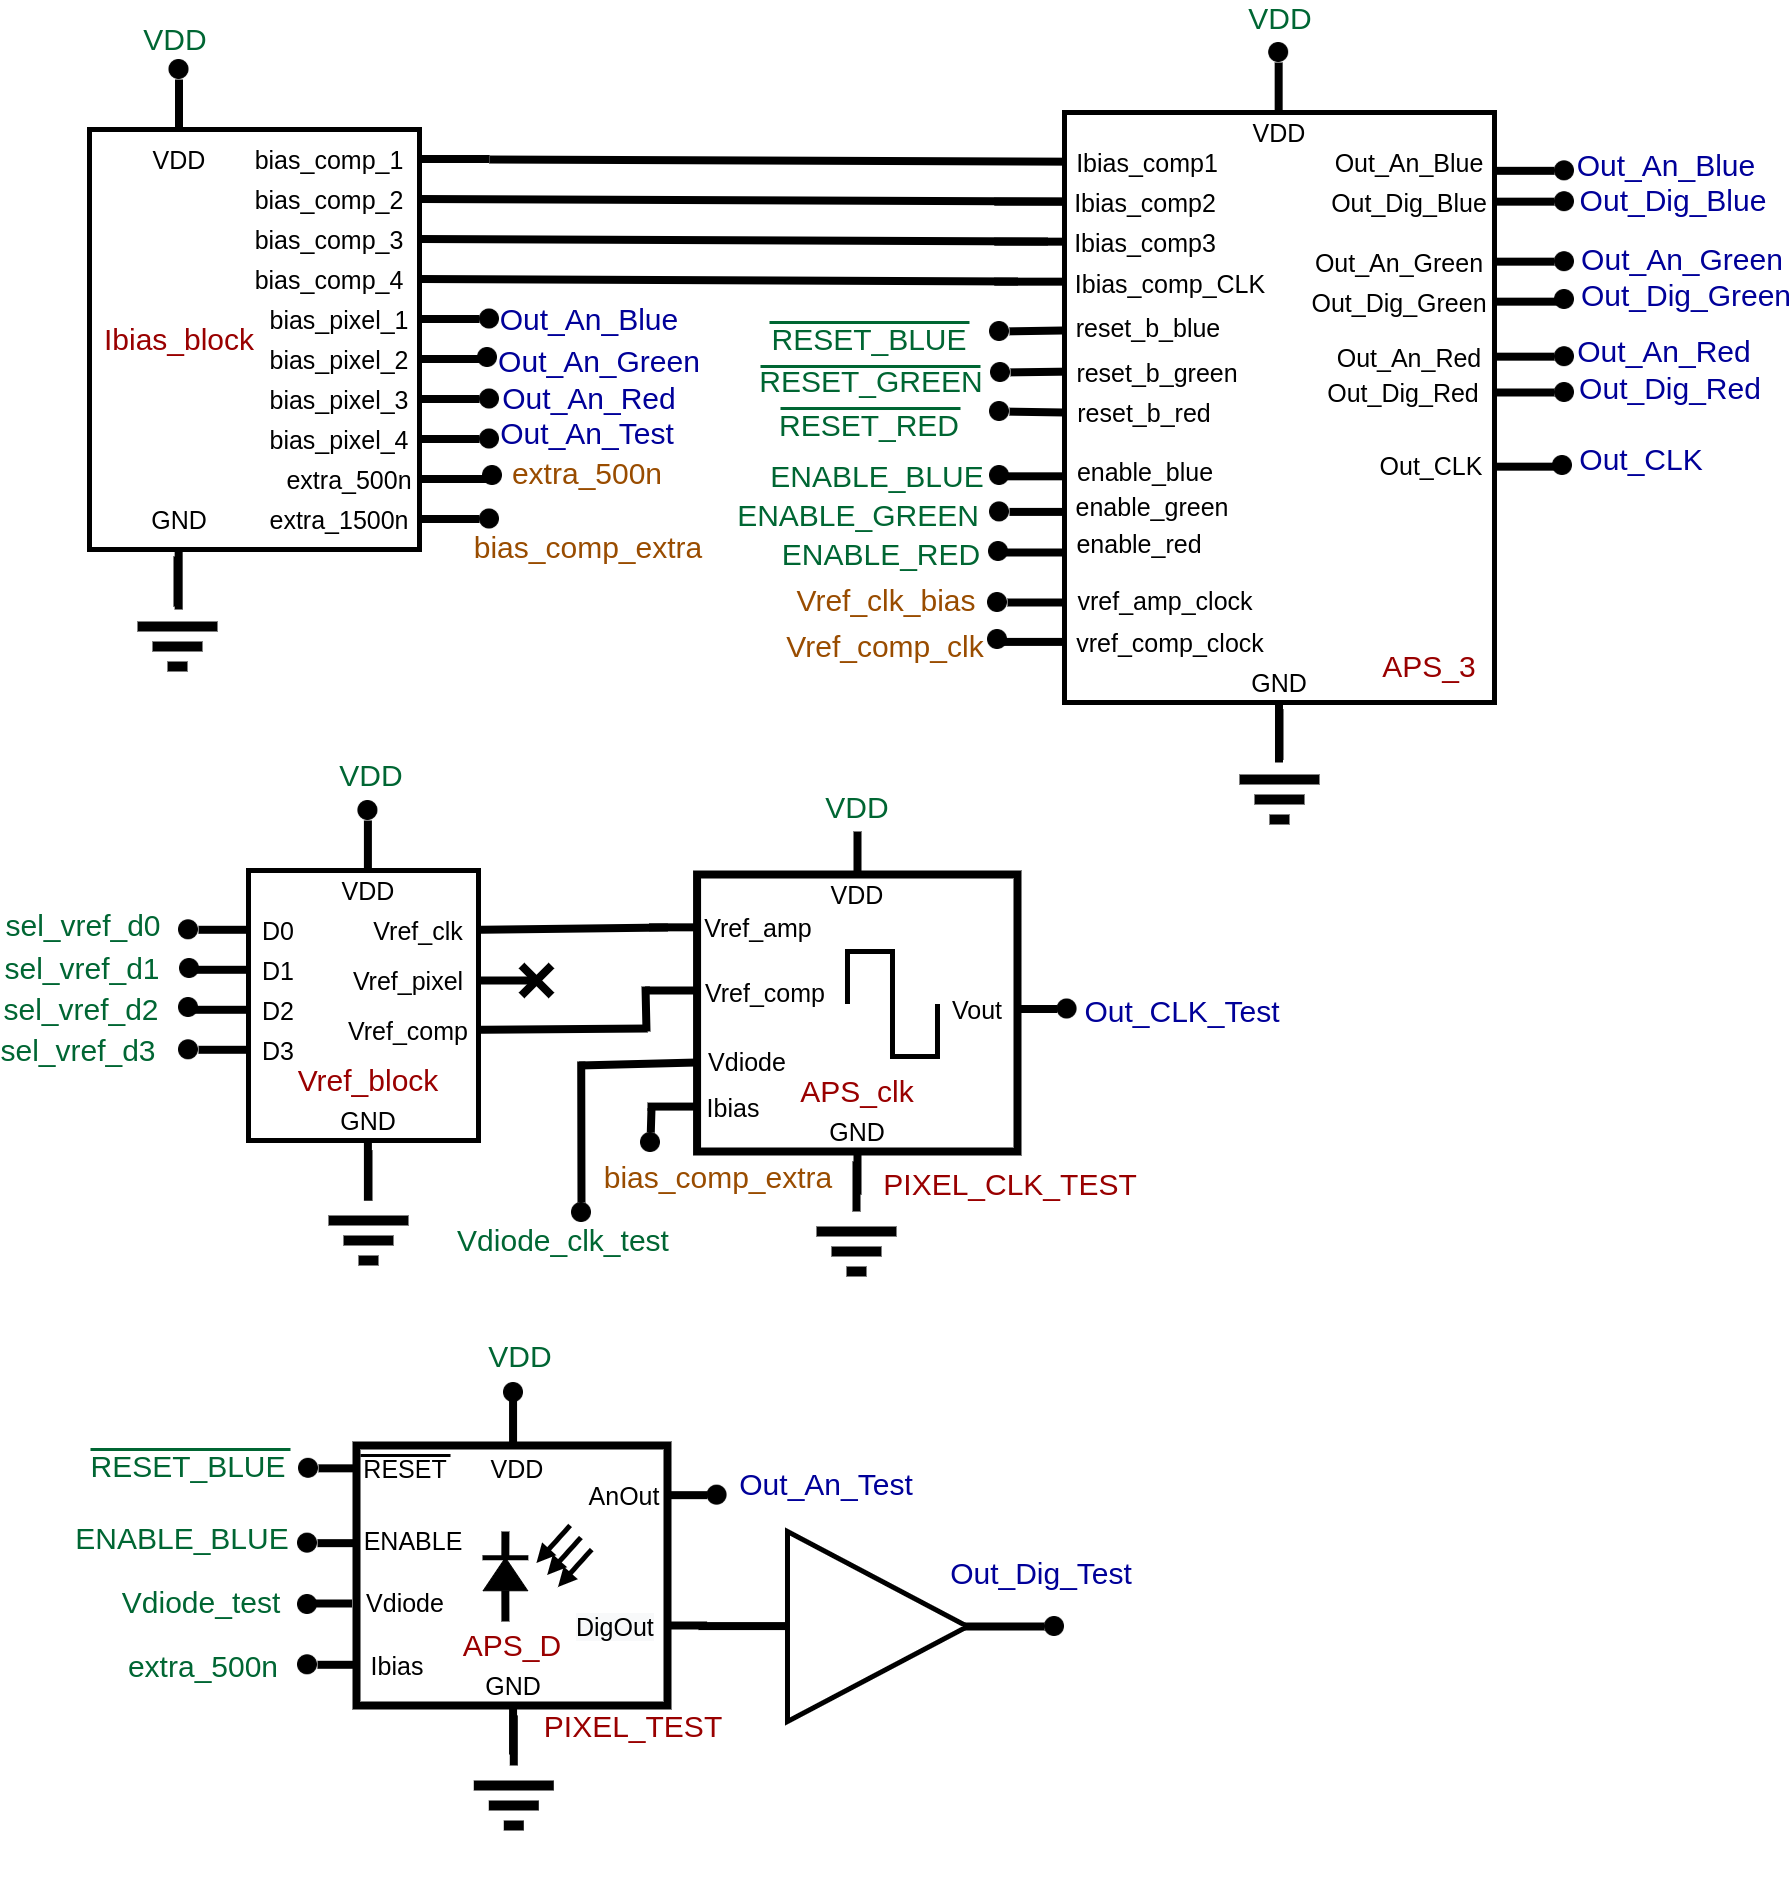
\includegraphics[width=\textwidth]{Circuitos/Complete_Circuit.png}
	\end{center}
	\legend{Fonte: Produzido pelo autor}
\end{figure}

\begin{figure}[!h]
	\caption{\label{fig_circcompletohigh}Representação dos principais blocos presentes no projeto}
	\begin{center}
	    \includegraphics[width=\textwidth]{Imagens/Complete_Circuit_rep.png}
	\end{center}
	\legend{Fonte: Produzido pelo autor}
\end{figure}


O circuito tem a finalidade de processar a informação advinda de tr\^es APS's, constru\'idos de maneira id\^entica em n\'ivel de layout, com a finalidade de abstrair informações de cores advindas de uma fonte luminosa, dos quais podem ser Azul, Verde ou Vermelha. Para que as cores fossem devidamente separadas, são utilizadas películas coloridas externas, que ficam acima de cada respectivo circuito APS de forma a permitir passar somente a informação de uma cor.

Um sinal luminoso de cor branca tamb\'em \'e utilizado no sistema de forma a ser a refer\^encia de rel\'ogio de todos APS's descritos. Esse sinal \'e processado utilizando-se um TIA, do qual \'e gerado um sinal el\'etrico equivalente \`a informação luminosa.

A tecnologia de fabricação utilizada para o desenvolvimento de todos blocos foi a \textit{CMOS TSMC 180nm}. O software utilizado para o projeto do dispositivo foi o \textit{Virtuoso}, desenvolvido pela empresa \textit{Cadence}.

O circuito representado na \autoref{fig_circcompleto} \'e composto por 2 blocos principais, que permitem o processamento advindos da fonte luminosa, al\'em de um circuito APS e um TIA extra. A descrição dos bloco são:

\begin{itemize}
    \item \textit{ibias\_block}: Tem a função de gerar fontes de corrente utilizadas em alguns blocos do circuito.
    
    \item \textit{APS\_3}: Implementa os tr\^es circuitos \textit{APS} descritos, al\'em do circuito TIA. A sa\'ida de cada bloco passa por um comparador de forma a digitalizar o dado, como ser\'a melhor explicitado na \autoref{sec_apsdigitalized}.
    
    \item \textit{Vref\_block} e \textit{PIXEL\_CLK\_TEST}: Estes blocos realizam a implementação de um TIA, por\'em com a adição de um pino extra que possibilita a simulação de uma corrente fotogerada sem necessitar de uma fonte luminosa. Estes blocos serão melhor explicados na \autoref{BlocoTestes}. 
    
    \item \textit{PIXEL\_TEST}: Este bloco realiza a implementação de um APS, com a adição de um pino adicional onde pode ser injetado uma corrente sem a necessidade de uma fonte luminosa. Este bloco será melhor explicado na \autoref{BlocoTestes}.
    
\end{itemize}

A \autoref{tab_circcomp2} mostra a relação de sinais de entrada e sa\'ida presentes no circuito para o processamento dos blocos de teste. A \autoref{tab_circcomp} mostra a relação de sinais de entrada e sa\'ida presentes no circuito, para o processamento dos p\'ixels de cor.

\begin{table}[ht]
  \caption{Descrição dos sinais de entrada e sa\'ida do circuito projetado para os blocos de teste}%
  \label{tab_circcomp2}
  \begin{tabular}{ccl}
  \toprule
   Sinal & Tipo & Descrição \\
   \midrule \midrule
   Vdiode\_test & Entrada & Corrente que simula um potencial no fotodiodo do APS de teste\\
   \midrule
   Vdiode\_clk\_test & Entrada & Corrente que simula um potencial no fotodiodo no TIA de teste\\
   \midrule
   Out\_An\_Test & Sa\'ida & Sinal de tensão anal\'ogico para o APS de teste \\
   \midrule
   Out\_Dig\_Test & Sa\'ida & Sinal de tensão digital para o APS de teste \\
  \midrule
   Out\_CLK\_test & Sa\'ida & Sinal de tensão de rel\'ogio gerado pelo TIA de teste\\
  \bottomrule
\end{tabular}%
  \legend{Fonte: Produzido pelo autor.}
\end{table}

\begin{table}[!h]
\centering
\caption{\label{tab_circcomp}Descrição dos sinais de entrada e sa\'ida do circuito projetado para as cores azul, verde e vermelha}%
  \begin{tabular}{ccll}
  \toprule
   Sinal & Tipo & Descrição & Observação \\
  \midrule \midrule
   RESET\_BLUE & Entrada & \begin{tabular}[l]{@{}l@{}}Sinal de tensão de \textit{RESET}\\ no APS para cor azul\end{tabular}   & Ativo em n\'ivel baixo \\
  \midrule
   RESET\_GREEN & Entrada & \begin{tabular}[l]{@{}l@{}}Sinal de tensão de \textit{RESET}\\ no APS  para cor verde\end{tabular}   & Ativo em n\'ivel baixo \\
  \midrule
   RESET\_RED & Entrada & \begin{tabular}[l]{@{}l@{}}Sinal de tensão de \textit{RESET}\\ no APS  para cor vermelha\end{tabular}   & Ativo em n\'ivel baixo \\
  \midrule
   ENABLE\_BLUE & Entrada & \begin{tabular}[l]{@{}l@{}}Sinal de tensão de \textit{ENABLE}\\ no APS para cor azul\end{tabular}   & Ativo em n\'ivel alto \\
  \midrule
   ENABLE\_GREEN & Entrada & \begin{tabular}[l]{@{}l@{}}Sinal de tensão de \textit{ENABLE}\\ no APS para cor verde\end{tabular}   & Ativo em n\'ivel alto \\
  \midrule
   ENABLE\_RED & Entrada & \begin{tabular}[l]{@{}l@{}}Sinal de tensão de \textit{ENABLE}\\ no APS para cor vermelha\end{tabular}   & Ativo em n\'ivel alto \\
  \midrule
   Out\_An\_Blue & Sa\'ida & \begin{tabular}[l]{@{}l@{}}Sinal de tensão anal\'ogica\\ para cor azul\end{tabular} \\
  \midrule
   Out\_Dig\_Blue & Sa\'ida & \begin{tabular}[l]{@{}l@{}}Sinal de tensão digital\\ para cor azul\end{tabular} \\
  \midrule
   Out\_An\_Green & Sa\'ida & \begin{tabular}[l]{@{}l@{}}Sinal de tensão anal\'ogica\\ para cor verde\end{tabular} \\
  \midrule
   Out\_Dig\_Green & Sa\'ida & \begin{tabular}[l]{@{}l@{}}Sinal de tensão digital\\ para cor verde\end{tabular} \\
  \midrule
   Out\_An\_Red & Sa\'ida & \begin{tabular}[l]{@{}l@{}}Sinal de tensão anal\'ogica\\ para cor vermelha\end{tabular} \\
  \midrule
   Out\_Dig\_Red & Sa\'ida & \begin{tabular}[l]{@{}l@{}}Sinal de tensão digital\\ para cor vermelha\end{tabular} \\
   \midrule
   Out\_CLK & Sa\'ida & \begin{tabular}[l]{@{}l@{}}Sinal de tensão de rel\'ogio\\ gerado pelo TIA\end{tabular}\\
  \bottomrule
\end{tabular}%

\legend{Fonte: Produzido pelo autor.}
\end{table}
